\section{Introduction}
A text detector observes a final passage. The process that produced it may include a human source, a model-generated draft, a second model's revision, or repeated revision by the original generator. These histories pose different questions. Detecting a machine intervention is different from identifying the first author, identifying the last generator, or establishing that a revision preserved the original claims. A binary detector score does not resolve all four questions.

This paper studies how fixed detector decisions change across sources and recorded production histories. The practical setting is a detector already fitted or calibrated on one collection and then applied to another. We preserve its operating point and ask what happens to both human false positives and machine-text sensitivity. We also hold the initial passage fixed while varying the rewriter, including a same-model second pass. This control matters because a large loss relative to direct generation may result from rewriting generally, without demonstrating a distinct advantage from crossing model families.

Previous work establishes that paraphrasing can impair detection, that benchmarks expose substantial variation across domains and generators, and that rewriting and conversational history can change model-attribution signals~\cite{sadasivan2023,dugan2024,perrone2026,yuan2026,tian2026}. We do not claim these observations as new. Our contribution is a complete, auditable empirical panel that combines three source-domain bundles, all nine ordered pairs of three model configurations, seven fixed detectors, a separate human-control cohort, and explicit accounting for unsuccessful completion of a length constraint. The panel supports comparisons that are easily obscured by a single pooled detection number.

Three questions organize the analysis. First, do operating points calibrated on human answers retain useful specificity on unrelated human material? Second, how do direct-generation and rewrite detection rates depend on the roles of the generator and rewriter? Third, how much of an apparent cross-model advantage remains visible when same-model rewriting and mechanical completion are examined? The third question is deliberately limited in this version: independent semantic-preservation ratings are pending, so the paper reports detector behavior and mechanical diagnostics, not a confirmed meaning-preserving attack.

The completed experiment contains 450 matched source items, 1,500 additional human controls, 6,750 model calls, and 60,900 scores. The comparison includes Binoculars, Fast-DetectGPT, and RADAR alongside four lightweight frozen classifiers. Every model output is scored, including outputs outside the prespecified length range. No outcome is regenerated because it is hard to detect, too short, too long, or otherwise inconvenient. All 357 source-specific binomial intervals are independently reconstructed from the score ledger.

The results show why these controls belong together. Character and style classifiers flag nearly all direct model outputs, but also flag many human controls. RADAR shows the opposite operating behavior: no false positives among the 1,500 controls, alongside low direct-generation sensitivity. Binoculars and Fast-DetectGPT are more selective, yet their sensitivity varies strongly with generator and rewrite history. For Gemma passages, both cross-model and same-model rewriting greatly reduce flags. Applying the prespecified length constraint changes the ordering of a diagnostic parent-positive-to-child-negative count. That count still lacks the semantic labels needed for the planned quality-qualified endpoint.

\section{Related Work and Scope}
\paragraph{Content detection and transport.}
Binoculars contrasts predictions from two related pretrained language models; Fast-DetectGPT uses a standardized discrepancy based on conditional token probabilities~\cite{hans2024,bao2024}. These methods provide substantive published comparators without fitting a new classifier to the present test panel. RADAR instead learns a detector through adversarial interaction with a paraphraser~\cite{hu2023}. We evaluate one released RADAR checkpoint and a specified Falcon reference pair for the two probability-based methods. Results for these implementations are not a ranking of every configuration of the three methods.

RAID evaluates detectors across generators, domains, decoding choices, and attacks~\cite{dugan2024}. We draw human source material from its nonadversarial training file and generate a new crossed panel. Thus, our experiment is neither the complete RAID benchmark nor a reproduction of its leaderboard. HC3 supplies the earlier fitting and human-only calibration environment~\cite{guo2023}. Moving from HC3 answers to RAID source-domain bundles changes subject matter, text conventions, and production task together. We call this \emph{transport}, without assigning the change to a single causal factor.

\paragraph{Rewriting and production history.}
Recursive paraphrasing and related attacks already challenge content detectors~\cite{sadasivan2023}. ARB explicitly matches human text, direct generation, human-origin rewriting, and same-generator rewriting~\cite{perrone2026}. Its construction provides a particularly close precedent for treating a second pass as an experimental condition. We extend the comparison across every ordered pair in a three-model panel while keeping same-model cells visible. Our smaller, differently sampled study cannot establish superiority over ARB or overturn its results under another calibration regime.

ForgePrint studies targeted transfer of model-attribution fingerprints and includes automated faithfulness controls~\cite{yuan2026}. Contagious Fingerprints examines model handoffs in conversation and introduces references conditioned on the same history~\cite{tian2026}. Those tasks differ from our fixed binary-detector evaluation, but both establish that a final stylistic signal need not authenticate the original production process. We do not propose a new attribution algorithm, a history-conditioned calibration method, or a trained rewriting attack. The contribution here is the measured behavior of frozen detectors under a fully enumerated, one-step rewrite design.

\paragraph{Calibration and inference.}
Order-statistic calibration offers marginal error control under exchangeability, not automatic protection against source shift~\cite{angelopoulos2021}. We retain that distinction. Binomial confidence intervals quantify sampling uncertainty under declared within-cell assumptions~\cite{clopper1934}; they do not repair a mismatch between the calibration and deployment populations. Neither framework licenses treating many descendants of one source item as independent observations.

\section{Experimental Design}
\subsection{Sources, exclusions, and sampling}
We use human-labeled, nonadversarial records from the official RAID \texttt{train\_none.csv} file in three domains: Wikipedia, scientific abstracts, and recipes. The complete 801,662,741-byte source file is pinned by SHA-256, and every selected record retains its original identifier and source-group identifier. Eligibility requires a nonempty source identifier, at least 60 whitespace-delimited words, and a nonempty title of at most 180 words. The title supplies a topic for direct generation; the human passage is not included in that prompt.

Before selection, the preparation routine checks previous training, development, calibration, evaluation, and smoke inputs from the local study series. It excludes matching source/question identifiers, normalized full-text and first-128-word hashes, and lexical near-duplicates. The near-duplicate rule is fixed at Jaccard similarity of at least 0.85 over five-word shingles after lowercase alphanumeric normalization of the first 128 whitespace-delimited words. The routine also screens newly admitted candidates against each other. These checks limit observed lexical reuse. They cannot establish absence from model pretraining or rule out semantic paraphrases.

A deterministic hash assigns five percent of eligible source groups to a separate smoke namespace. Full-study selection uses the remaining namespace. Each domain supplies 150 matched experimental source items and a disjoint set of 500 human controls. The available full-study pools contain 1,698 Wikipedia groups, 1,659 abstract groups, and 1,695 recipe groups, each exceeding the required 650. The design fails if a source cannot provide its planned count; it does not silently shrink a difficult stratum.

The first 128 words of each selected human passage, or the whole passage when shorter, are retained as an excerpt. The 450 excerpts associated with the matched experiment are \emph{human references}. They provide parents for human-origin rewriting and are reported separately from the 1,500 controls used to describe false positives. The original corpus's human label is inherited. We did not observe these texts being written, recruit their authors, or establish author independence across source records.

\subsection{A complete ordered production matrix}
Let $i$ index a matched source item and let $a,b\in\{Q,L,G\}$ denote the installed Qwen, Llama, and Gemma configurations. We obtain a direct passage $D_{ia}$ from each generator. Each passage is then rewritten once by every configuration, yielding $R_{iab}$. The diagonal $R_{iaa}$ is the same-model control. Separately, each configuration rewrites the human reference $H_i$, yielding $U_{ib}$. Every matched item therefore contributes three direct calls, nine model-origin rewrite calls, and three human-origin rewrite calls.

\begin{table}[t]
\centering
\caption{Completed observation inventory. Human references and separate controls have different roles.}
\label{tab:inventory}
\begin{tabular}{lrr}
\toprule
Condition & Per source & Total\\
\midrule
Separate human controls & 500 & 1,500\\
Matched human references & 150 & 450\\
Direct generations & 450 & 1,350\\
Model-origin rewrites & 1,350 & 4,050\\
Human-origin rewrites & 450 & 1,350\\
\midrule
All scored texts & 2,900 & 8,700\\
Model calls & 2,250 & 6,750\\
\bottomrule
\end{tabular}
\end{table}

Direct prompts request a self-contained explanatory passage of 110--125 words on the source title, in prose rather than a list. Rewrite prompts request new wording and sentence organization while preserving every material assertion, adding no assertions, and omitting no material information. The same length target applies. This is a single fixed rewriting instruction, with no detector feedback, candidate search, or model-specific prompt tuning. It is not an optimized adversarial attack.

The mechanical completion contract allows 100--128 words, a completed request, and a termination reason other than an output limit. The target and acceptance range are distinct. A request that completes normally can still violate the word-count contract. Failed or incomplete outcomes were to remain recorded, and missing parents were to produce dependent-missing child records. Actual execution completed every planned call. All direct parents were available before their children; immutable parent identifiers and text hashes link the chain.

\subsection{Models and execution}
The three installed tags are \texttt{qwen3.5:4b}, \texttt{llama3.1:8b}, and \texttt{gemma4:12b}. Model digests, architecture metadata, serving version, and request configurations are recorded before generation. We refer to these as Qwen, Llama, and Gemma for readability, but the claims concern these pinned installations. Qwen and Gemma use an MLX runner; Llama uses a GGUF/GGML configuration. Qwen reports NVFP4, Llama reports Q4\_K\_M, and the Gemma metadata does not report a quantization label. These differences prevent an architecture-only or parameter-count-only interpretation.

The request client sets temperature 0.7, top-$p$ 0.9, repetition penalty 1.0, an 8,192-token context, and at most 384 output tokens. Thinking is disabled where the serving interface supports that option, and only the final response field is analyzed. Deterministic seeds and request identities support replay and caching, without assuming bitwise determinism across hardware or future server versions. The local server reports version 0.40.13. No generation model is trained or updated in this experiment.

\subsection{Detector panel and calibration}
Three lightweight classifiers use word unigrams/bigrams, character 3--5-grams, or eight length/style features. The features are log word count, log character count, mean word length, lowercase type-token ratio, and digit, punctuation, uppercase, and sentence-boundary frequencies. They were fitted in the preceding local study on 80 HC3 question groups, using one human answer per group and direct Qwen and Llama outputs. A fourth classifier, historical word TF-IDF, uses the same human groups and their historical HC3 machine answers. TF-IDF vocabularies are limited to 50,000 features; logistic regression uses balanced class weights and fixed $C=1$. No classifier is refitted here. Gemma outputs were absent from their fitting and development stages. This is an operation-specific holdout, not evidence that all pretrained components are unfamiliar with the Gemma lineage.

Binoculars and Fast-DetectGPT use the pinned Falcon-7B observer/reference model and Falcon-7B-Instruct performer/scoring model. Both employ the original published score functions. Native bfloat16 forward passes run on Apple MPS, followed by float32 CPU score reductions. A numerical-parity guard in the preceding setup rejected an algebraically equivalent reduction; the production version invokes the pinned original functions directly. The present panel uses that corrected, frozen implementation. Binoculars flags lower scores; Fast-DetectGPT flags higher scores. Sharing a Falcon pair makes their errors potentially dependent.

RADAR uses the released \texttt{TrustSafeAI/RADAR-Vicuna-7B} checkpoint at a pinned revision. This checkpoint is a RoBERTa-based detector; its name identifies its training setting, not a seven-billion-parameter detector architecture. We take the published class-zero probability as the machine-text score. RADAR was specified as an additional comparator before this panel's evaluation and completed all observations. It does not supply ground truth for the other methods.

Every method uses a separately determined threshold on the same 500 held-out human HC3 ELI5 answers. After orienting scores so that larger values indicate machine evidence, the cutoff is the 476th order statistic, $\lceil(500+1)0.95\rceil$, and ties at the cutoff are not flagged. This is a five-percent marginal false-positive target under calibration/test exchangeability. It is not a guarantee for the three new domains. Raw cutoffs are 0.8635380864 for Binoculars, 1.9734587669 for Fast-DetectGPT, and 0.9960119724 for RADAR, with the corresponding score directions. Published benchmark thresholds are not transferred to this study.

All detector inputs are the first 128 whitespace-delimited words, with whitespace normalized. The pretrained detectors additionally cap their tokenized input at 512 tokens; that extra cap binds for none of the recorded texts. No chat template is applied to detector inputs. Human-origin rewriting receives the retained excerpt, not the entire original corpus document. Generated parents and children may exceed 128 words. The planned semantic review concerns their full recorded texts, so the scope of a detector observation and the scope of the fidelity judgment remain distinct.

\section{Measurements and Statistical Scope}
Let $F_d(x)\in\{0,1\}$ be detector $d$'s frozen decision on the observed prefix of text $x$. For each source $s$, the human-control false-positive estimate is
\begin{equation}
\widehat{\mathrm{FPR}}_{ds}=\frac{1}{500}\sum_{i\in\mathcal H_s}F_d(H_i).
\end{equation}
Direct and rewrite flag rates use their planned 150-item source cells. For a particular pair $(a,b)$, we also record lost flags, $F_d(D_{ia})=1$ and $F_d(R_{iab})=0$, and gained flags with the reverse transition. Their difference reconciles the change in the marginal flag rate. These are paired descriptions of one question/source group, not independent samples of parents and children.

The frozen family contains seven detectors, three sources, and 17 conditions per source: one human-control cell, one human-reference cell, three direct cells, nine rewrite cells, and three human-origin rewrite cells. We retain all $7\times3\times17=357$ cells. Each two-sided Clopper--Pearson interval uses tail probability $0.05/(2\times357)$~\cite{clopper1934}. Bonferroni's union bound supplies simultaneous coverage under the binomial assumptions within each cell without requiring independence across detectors or conditions. The assumptions still require an appropriate independent-source-group sampling interpretation within a cell. Repeated authors and unobserved source dependence can violate that interpretation.

All planned texts are successfully scored. Thus, there is no distinction between planned and scored denominators in the completed rate tables. Mechanical length failures remain in those denominators. The interval family was specified before the full-panel detector results. The final audit independently reconstructs every numerator, denominator, and interval from stored decisions and verifies each decision against its frozen score cutoff.

Pooled counts use equal source weights because the three strata have equal sample sizes. They are descriptive summaries. In particular, the 1,350 direct outputs contain three descendants of each of 450 source items, and the 4,050 rewrites contain nine. We do not attach independent-binomial intervals to these pooled counts. The full ordered matrix, raw score changes, and highlighted cross-versus-self comparisons are reported without new significance tests or post hoc selection of a winning detector. Source-specific intervals are available for every cell; no confidence bound for a quality-qualified endpoint is reported before its labels exist.

\section{Results}
\subsection{Specificity and sensitivity must be read together}
Table~\ref{tab:detectors} reports all seven comparators. The word classifier flags 24 of 1,500 human controls, but only 120 of 1,350 direct generations. Character TF-IDF flags 1,347 direct generations while also flagging 1,465 human controls. The length/style classifier flags 1,342 direct generations and 994 human controls. Those high direct-generation rates cannot be interpreted as useful origin discrimination without the accompanying specificity results.

\begin{table*}[t]
\centering
\caption{Frozen operating points on new source-domain bundles. Human entries are false positives out of 500 controls per source. Direct-generation counts pool three models and three sources and are descriptive because outputs share source items.}
\label{tab:detectors}
\begin{tabular}{lrrrrr}
\toprule
Detector & Wikipedia & Abstracts & Recipes & Human total / 1,500 & Direct total / 1,350\\
\midrule
Word TF-IDF & 0 & 2 & 22 & 24 (1.60\%) & 120 (8.89\%)\\
Character TF-IDF & 482 & 483 & 500 & 1,465 (97.67\%) & 1,347 (99.78\%)\\
Length/style & 362 & 495 & 137 & 994 (66.27\%) & 1,342 (99.41\%)\\
Historical word & 69 & 234 & 5 & 308 (20.53\%) & 635 (47.04\%)\\
Binoculars & 9 & 11 & 22 & 42 (2.80\%) & 738 (54.67\%)\\
Fast-DetectGPT & 9 & 16 & 12 & 37 (2.47\%) & 767 (56.81\%)\\
RADAR & 0 & 0 & 0 & 0 (0.00\%) & 63 (4.67\%)\\
\bottomrule
\end{tabular}
\end{table*}

Binoculars flags 9 Wikipedia, 11 abstract, and 22 recipe controls. Fast-DetectGPT flags 9, 16, and 12. Their observed rates remain below five percent in all three sources, but this is an empirical observation, not a transported conformal guarantee. RADAR flags no human controls in any source. For zero of 500 observations, the upper endpoint in the 357-cell family is 1.895\%, rather than zero. This conservative source-specific bound concerns the sampled population under the stated assumptions, not every human writing style.

RADAR's low false-positive behavior coexists with 63/1,350 direct-generation flags. It therefore illustrates a restrictive operating point, not a universal solution to transport. Conversely, the character and style classifiers illustrate how apparent sensitivity can come from a decision rule that also rejects ordinary human material. The historical-word detector is intermediate, with particularly high human false positives on abstracts. Since the classifiers are frozen and the test task differs from their fitting environment, these results describe deployment mismatch rather than their best achievable retrained performance.

\begin{figure*}[t]
\centering
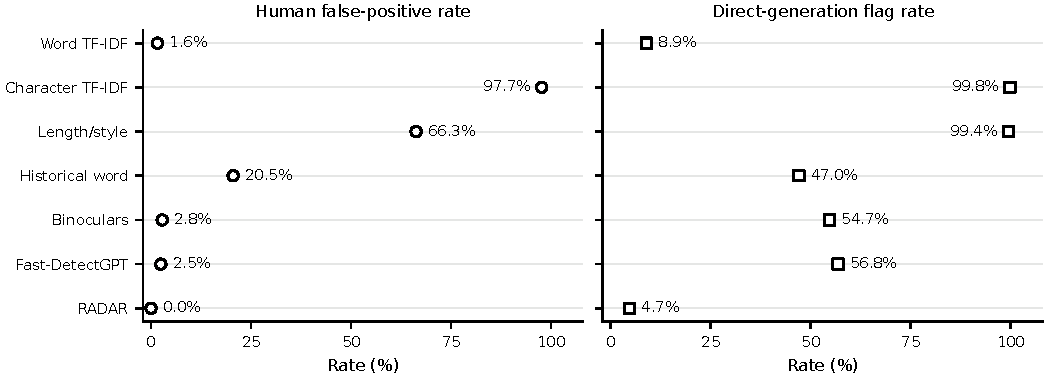
\includegraphics[width=\textwidth]{figures/detector_operating_points.pdf}
\caption{Human specificity and direct-generation sensitivity at the same frozen operating points. Left: pooled false-positive rates for 1,500 human controls. Right: pooled flag rates for 1,350 direct generations. Both panels are descriptive point estimates, with equal source weights; the right panel also equally weights the three models. No confidence intervals are shown. Source-specific intervals retain the fixed 357-cell family in the accompanying tables.}
\label{fig:operating}
\Description{Seven detector rows compare pooled human false-positive rates with pooled direct-generation flag rates. Character and style classifiers show high rates on both human and generated text. RADAR has zero human flags and low direct-generation sensitivity.}
\end{figure*}

\subsection{Direct-generation sensitivity varies by model}
For Binoculars, the direct counts are 35/450 for Qwen, 448/450 for Llama, and 255/450 for Gemma. Fast-DetectGPT yields 57/450, 447/450, and 263/450. The same fixed scoring pair and calibration rule therefore produce very different decisions across the three installed generators. RADAR flags 0/450 Qwen, 37/450 Llama, and 26/450 Gemma passages. The word classifier favors a different ordering, flagging 100 Qwen, three Llama, and 17 Gemma passages.

The differences are also source dependent. Binoculars flags 125/150 direct Gemma passages from Wikipedia topics, 33/150 from abstract topics, and 97/150 from recipe topics. Fast-DetectGPT yields 126/150, 42/150, and 95/150. These contrasts concern topic-conditioned generated passages, not the original human passages. Model family, decoding implementation, output length, and source-specific task suitability are not experimentally isolated. The results establish heterogeneity in this panel, rather than its cause.

\subsection{The full rewrite matrix includes increases as well as losses}
Figure~\ref{fig:matrix} includes every ordered pair and all seven methods. Rewriting does not uniformly decrease flags. Binoculars flags 35 direct Qwen passages but 138 of their Llama rewrites; Fast-DetectGPT changes from 57 to 147. Gemma-to-Llama counts are 256 for Binoculars and 262 for Fast-DetectGPT, close to the direct Gemma counts of 255 and 263. The reverse Llama-to-Gemma direction yields 150 and 162, respectively, versus 448 and 447 direct Llama flags. The direction of the production edge matters.

Same-model rewriting also changes detection. Binoculars flags four Qwen self-rewrites, 388 Llama self-rewrites, and 44 Gemma self-rewrites. Fast-DetectGPT flags 11, 390, and 52. Thus, a second pass by the initial generator can substantially alter a detector decision. Character and style flags, meanwhile, remain near saturation across much of the matrix, consistent with their poor human specificity. The full panel prevents selective emphasis on only the cells with a visually large reduction.

\begin{figure*}[t]
\centering
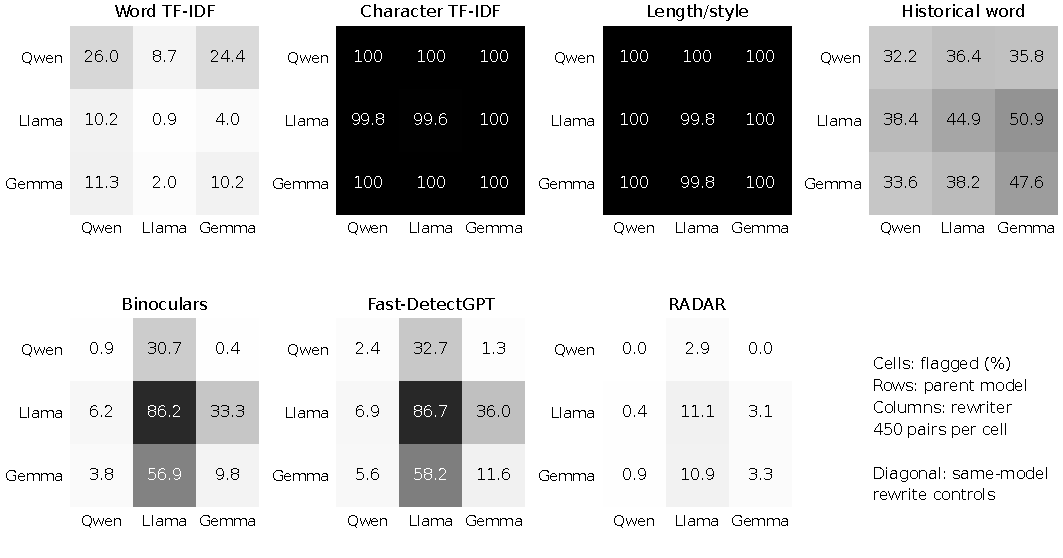
\includegraphics[width=\textwidth]{figures/rewrite_matrix_all.pdf}
\caption{All ordered generator--rewriter pairs, with 450 matched items per cell. Rows indicate the parent generator; columns indicate the rewriter. Diagonal cells are same-model controls. Each percentage is a descriptive detector flag rate, not meaning-preserving attack success. All outcomes remain included. Source-specific matrices and exact counts accompany the analysis.}
\label{fig:matrix}
\Description{Seven three-by-three grayscale matrices show rewrite flag percentages for each detector. Rows are Qwen, Llama and Gemma parents, and columns are the three rewriters. Same-model diagonals and asymmetric cross-model edges are visible.}
\end{figure*}

\subsection{A same-model control changes the primary-arm interpretation}
The preselected quality-review contrast compares Gemma-to-Qwen with Gemma-to-Gemma. Before any semantic judgment, Binoculars flags 255/450 direct Gemma passages, 17/450 Qwen rewrites, and 44/450 Gemma self-rewrites. Fast-DetectGPT gives 263, 25, and 52. The direct-to-Qwen decrease is large, but the difference between the two final rewrite flag rates is only 27/450, or six percentage points, for each detector. These are different contrasts and must not be substituted for each other.

A further distinction arises when requiring that the parent was actually flagged. Binoculars has 238 parent-positive-to-child-negative transitions for Qwen rewrites and 212 for self-rewrites. Fast-DetectGPT has 238 and 214. The same-model counts differ from simple marginal losses because some initially unflagged parents gain a flag after rewriting. Retaining parent identifiers allows those transitions to be reconciled exactly.

Applying only the frozen mechanical length/completion rule gives 196 versus 210 for Binoculars and 198 versus 212 for Fast-DetectGPT (Table~\ref{tab:primarydiagnostic}). The ordering reverses in this diagnostic. Neither row is the planned quality-qualified endpoint: preserving length is not preserving meaning. Nor does this establish that semantic review must produce a particular result. It does show that a direct-to-cross detection drop cannot be reported as a completed quality-preserving advantage.

\begin{table}[t]
\centering
\caption{Diagnostics for the preselected Gemma-parent arms. Cross denotes a Qwen rewrite and self a Gemma rewrite. Every entry uses the same 450 planned source items. None incorporates semantic-preservation labels or constitutes the primary endpoint.}
\label{tab:primarydiagnostic}
\small
\begin{tabular}{lrrrr}
\toprule
 & \multicolumn{2}{c}{Binoculars} & \multicolumn{2}{c}{Fast-DetectGPT}\\
Quantity & Cross & Self & Cross & Self\\
\midrule
Child flagged & 17 & 44 & 25 & 52\\
Parent flagged, child not & 238 & 212 & 238 & 214\\
Above + mechanical rule & 196 & 210 & 198 & 212\\
\bottomrule
\end{tabular}
\end{table}

\subsection{Human-origin rewriting is a separate condition}
Human-origin rewrites are not human-negative controls. Each has a recorded model intervention, although its parent carries a human corpus label. On the 450 human-reference parents, Binoculars and Fast-DetectGPT each flag 11. Qwen rewrites of these parents receive zero flags from either method. Llama rewrites receive 118 Binoculars flags and 96 Fast-DetectGPT flags; Gemma rewrites receive 12 and eight. RADAR flags one Llama rewrite and no Qwen or Gemma rewrite.

These outcomes reinforce the distinction between detecting an intervention and identifying the origin of the underlying claims. They do not prove that an unflagged rewrite is fully human-authored, faithful, or factually correct. The machine-intervention history is known from execution, while the content relationship requires a different measurement. All other detector results for this condition, including the high character and style flag rates, are retained in the accompanying tables.

\subsection{Completion, length, and execution cost}
All 6,750 generation calls finish, and all 60,900 detector scores are finite and recorded without scoring errors. There are no unrun generation slots, missing detector pairs, or output-token-limit terminations. Nonetheless, 1,483 generated passages, 21.97\%, violate the 100--128-word contract: 599 are short and 884 are long. The additional 512-token detector cap does not bind, but the common 128-word prefix rule necessarily omits the suffix of overlength texts.

Length compliance differs markedly by configuration. Qwen meets the contract in 63/450 direct generations, 795/1,350 model-origin rewrites, and 275/450 human-origin rewrites. The corresponding Llama counts are 436, 1,200, and 334; Gemma yields 450, 1,306, and 408. These differences make it inappropriate to read a detector contrast as an isolated model-family effect. The figures and tables retain every planned outcome rather than selecting a length-compliant subset for a favorable headline.

\begin{figure}[t]
\centering
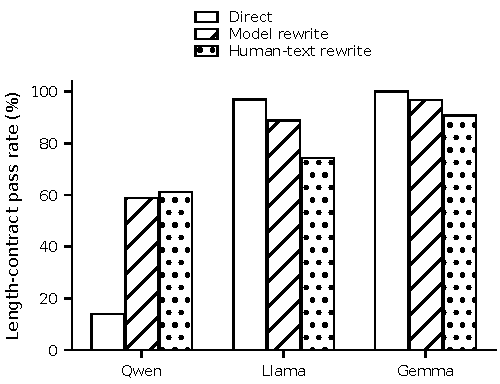
\includegraphics[width=\columnwidth]{figures/length_compliance.pdf}
\caption{Mechanical completion by final model and operation. All planned generations are included. Meeting the word-count range does not establish fidelity or factual correctness.}
\label{fig:length}
\Description{Grouped bars compare the fraction meeting the fixed word-count contract for direct generation, model-origin rewriting and human-origin rewriting. Qwen compliance is lowest, especially for direct generation.}
\end{figure}

A prespecified phrase heuristic flags five possible refusals, all in human-origin rewrites. These flags remain unadjudicated and are not treated as verified refusal labels. There are 22 normalized first-128-word collision groups, all within the same source item; no cross-item collision is observed. Repeated outputs are retained rather than selectively removed.

The recorded generation stage takes 10,746 seconds, approximately 2.99 hours, and detector scoring takes 2,152 seconds, approximately 35.9 minutes, on the local Apple system. Generation records contain 1,511,883 prompt tokens and 953,238 output tokens. These measurements describe one invocation and its serving configuration. They exclude initial model downloads and do not constitute a matched throughput comparison among models or detector methods.

\section{The Pending Quality-Qualified Analysis}
The protocol includes a prospective semantic-review endpoint, which is not yet observed. For detector $d$ and rewrite condition $b$, define
\begin{equation}
J_{idb}=F_d(D_{iG})[1-F_d(R_{iGb})]M_{ib}V_{ib},
\end{equation}
where $M_{ib}$ records independently reviewed preservation of the parent's material content, and $V_{ib}$ records valid completion under the frozen rubric, including the mechanical length constraint. An initial parent that is not flagged contributes zero. Every planned source item remains in the denominator, avoiding a success estimate restricted to detectable parents or completed high-quality outputs.

The two directional primary claims concern Binoculars and Fast-DetectGPT separately. Each asks whether the equally source-weighted difference between Gemma-to-Qwen and Gemma-to-Gemma $J$ exceeds ten percentage points. The margin is an investigator-selected design criterion, not an established literature constant. Each claim uses a one-sided 97.5\% lower bound. The frozen method is a source-stratified paired studentized approximation with Welch--Satterthwaite degrees of freedom. It falls back to conservative weighted source-specific paired-discordance Clopper--Pearson bounds if a source has fewer than 30 items, fewer than five cross-only or same-only successes, or degenerate variance. The conservative calculation is always reported as a sensitivity analysis. No exact finite-sample coverage claim is made for the studentized approximation.

The review packet contains 900 primary parent--rewrite pairs and 12 synthetic attention controls per reviewer. Two independent reviewers are to assess each pair without detector scores, model identities, or the experimental arm labels; disagreements and uncertain judgments require adjudication before analysis. Fidelity is judged relative to the parent, which may itself be factually wrong. It is not a claim of external factual verification. Attention-control outcomes will be reported without inventing a post hoc exclusion rule.

As of this version, no locked annotation file exists and no quality-qualified effect estimate, confidence bound, or acceptance verdict is available. The raw and mechanical counts in Table~\ref{tab:primarydiagnostic} cannot fill that gap. Completion of this review would support an updated analysis under the existing protocol; changing prompts, margins, or test items after inspecting these results would require a separate study.

\section{Validity, Interpretation, and Reproducibility}
\paragraph{A bounded transport claim.}
The calibration set consists of HC3 ELI5 answers, whereas evaluation combines human material and title-conditioned prose from three RAID domains. Genre, topic, source, text length, and task change together. Human and direct model passages are topically linked but are not semantically matched answers produced under identical instructions. The study therefore measures deployment behavior on a specified bundle of changes. It does not isolate demographic bias, demonstrate that a detector fails on every source, or establish that the human and model distributions have converged.

\paragraph{A bounded history claim.}
The full matrix exposes asymmetric transitions and provides same-model controls. It does not independently vary model size, quantization, training ancestry, decoding backend, or rewrite strength. Only three configurations and one rewriting instruction are tested, with one draw per item and condition. Nine ordered cells do not create nine independent model families. Repeated descendants share their parent, and shared reference models can correlate detector errors. The analysis preserves those dependencies in its data structure and avoids treating pooled generations as independent binomial trials.

\paragraph{Quality and observation boundaries.}
A detector sees a prefix; the planned reviewer will assess full recorded model passages. Long generated parents can make the fixed-length rewrite instruction demand compression even while asking for preservation of every material assertion. Human-origin rewrites receive at most 128 words of the original source, so any preservation claim for that condition would concern the retained excerpt, not the complete source document. The experiment cannot establish semantic fidelity from an instruction, a lexical-overlap score, a completed API call, or a detector's negative decision. Length and refusal diagnostics describe observable compliance problems without replacing the pending judgment.

\paragraph{Study sequence and analytical restraint.}
This panel was designed after an earlier HC3 detector study. It is a new source-item panel with locally frozen manifests and analysis rules, not an independent conception of the research questions or an externally registered study. The three published detector implementations, their human calibration data, and the lightweight classifier weights were fixed before scoring this extension. Final reporting reproduces the stored cell family and introduces no new hypothesis tests. Highlighting particular cells is descriptive; the full matrix and all source tables permit examination of contrary outcomes.

\paragraph{What the experiment can contribute.}
The informative result is not simply that rewriting sometimes reduces a score. First, a detector's low false-positive count and its sensitivity to different generators must be reported together. Second, a direct-to-cross comparison can overstate the evidence for a cross-model advantage if self-rewriting produces a similar loss. Third, mechanical validity can change the ordering of a seemingly favorable comparison before semantic quality is considered. These observations motivate complete history controls and planned-denominator reporting. They do not introduce a new detector, prove an impossibility theorem, authenticate an author, or validate watermark removal.

\paragraph{Reproducibility and use.}
The accompanying artifact records source identifiers, input hashes, generator digests, frozen thresholds, parent links, detector decisions, and analysis code. A separate audit reconstructs the condition inventory and 357 intervals while verifying completion snapshots and source hashes. The code distribution can reproduce aggregate analyses from metadata and scores without redistributing source prose, model weights, private review mappings, or reviewer identities. Source texts and model checkpoints retain their original licenses, including the RADAR checkpoint's research-use restrictions. Availability of a code repository should not be read as permission to redistribute every upstream asset.

The observations support detector evaluation, not an automated accusation against a writer. The false-positive counts are inherited-corpus measurements and contain no new consented authorship observations. A negative score is not proof of human authorship, and a positive score does not identify the complete production chain. Research that needs stronger provenance claims must measure the missing process information rather than infer it from the present binary outputs.

\section{Conclusion}
A completed three-source, three-model experiment yields different answers depending on whether the question concerns human specificity, direct-generation sensitivity, a rewrite edge, or a same-model control. Across seven frozen detectors, the study records both severe specificity failures and conservative low-sensitivity behavior. The full ordered matrix reveals losses, increases, and substantial same-model changes. For the preselected Gemma-parent comparison, a large direct-to-Qwen decline does not by itself establish a cross-model advantage, and length compliance materially changes the relevant diagnostic counts. All 6,750 generations and 60,900 scores are complete; the semantic-review endpoint remains pending. The defensible result is an audited account of detector transport and recorded rewrite histories, with the boundary between observed detector behavior and unmeasured content preservation kept explicit.
